\begin{frame}[parent={ie:agenda}, hasnext=true, hasprev=false]
	\frametitle{Modelo espiral}

	\begin{block:concept}{Definição}
		Modelo de ciclo de vida iterativo e baseado em riscos~\cite{Boehm:1986, Boehm:1988}.
	\end{block:concept}
	
	\begin{block:fact}{Contexto}
		\begin{itemize}
			\item Desenvolvimento de projetos governamentais (provavelmente relacionado
			a projetos para desenvolvimento de software para planejamento, comando e
			análise pós-vôo de missões espaciais na TRW).
			
			\item \~ 1980
		\end{itemize}
	\end{block:fact}
	
	\note{
		\begin{itemize}
			\item Modelo baseado em riscos em contraposição aos modelos baseados em
			documentação e codificação de outrora.
			
			\item Foi criado a partir da experiência no uso e em alterações do modelo
			cascata com retornos (figura do Royce, modelo de outro autor)~\cite{Boehm:1976}.
			
			\item \textbf{Não é necessariamente incremental, dado que não temos um produto
			executável a cada iteração}.
		\end{itemize}
	}
\end{frame}


\begin{frame}[hasnext=true, hasprev=true]
	\frametitle{Modelo espiral}

	\begin{block:fact}{}
		\centering
		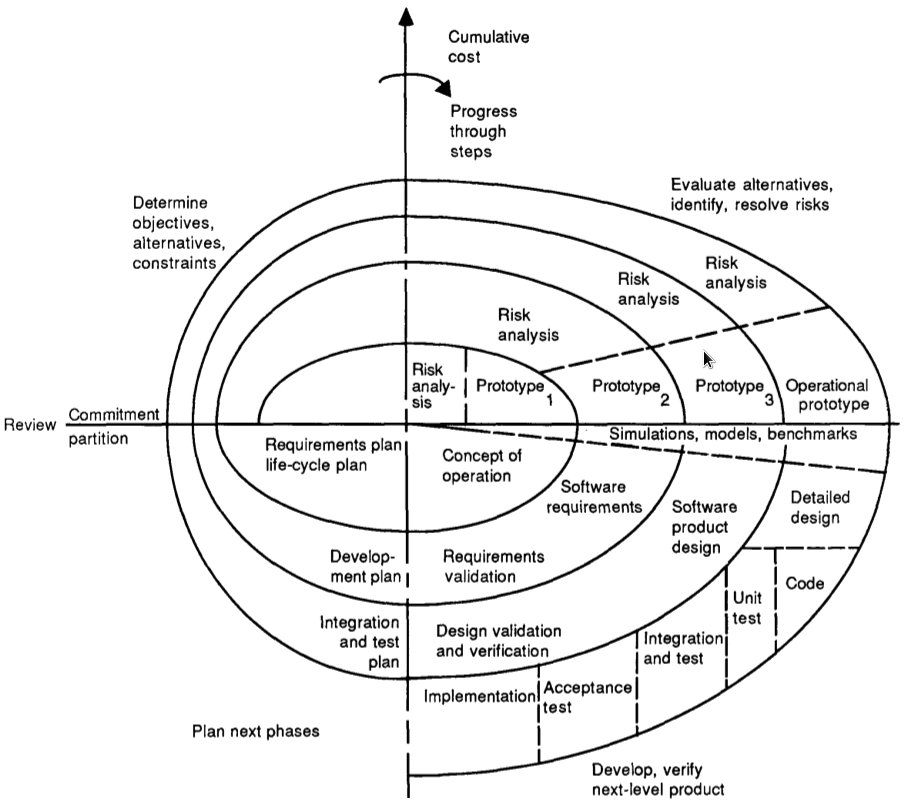
\includegraphics[width=.8\textwidth]{software-engineering/project-management/process/sdlc/spiral/spiral}
	\end{block:fact}
	
	\note{
		\begin{itemize}
			\item Raio = custo acumulativo
			\item Ângulo = progresso para completar o ciclo/iteração
		\end{itemize}
	}
\end{frame}


\begin{frame}
	\frametitle{Modelo espiral}
	\framesubtitle{Primeiro quadrante}

	\begin{columns}
		\column{.48\textwidth}
		\begin{block:fact}{Primeiro quadrante}
			\begin{itemize}
				\item Determinar objetivos do produto.
				\item Identificar restrições.
				\item Identificar alternativas para alcançar os objetivos.
			\end{itemize}
		\end{block:fact}

		\column{.48\textwidth}
		\begin{block:fact}{}
			\centering
			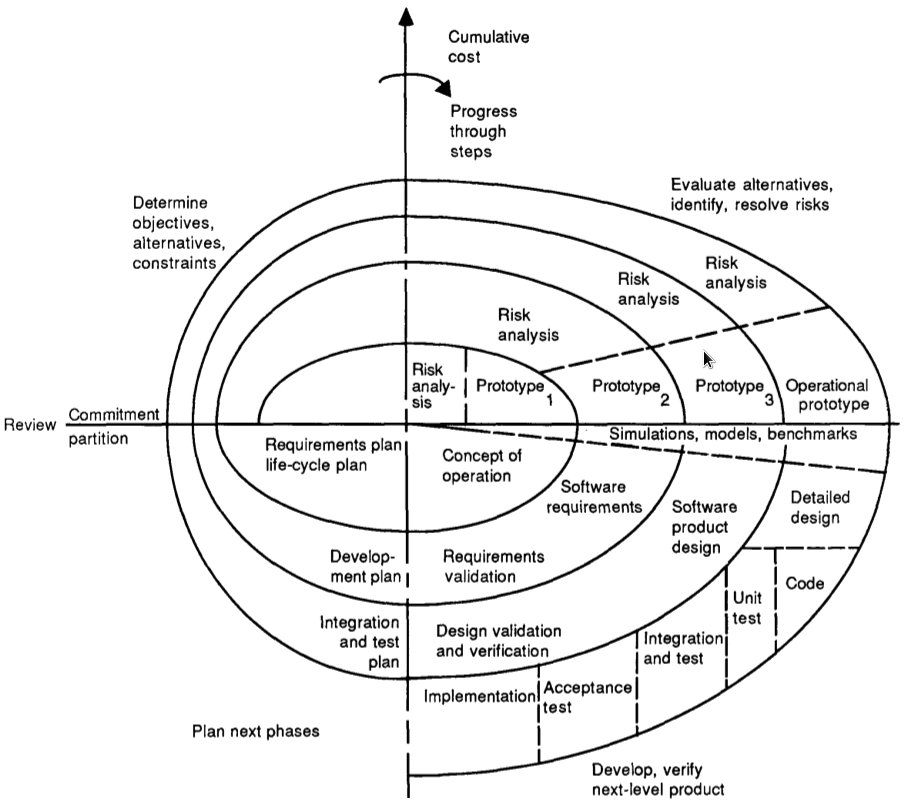
\includegraphics[width=\textwidth]{software-engineering/project-management/process/sdlc/spiral/spiral}
		\end{block:fact}
	\end{columns}
	
	\begin{block:fact}{Objetivos do produto}
		\begin{itemize}
			\item Objetivos organizacionais
			\item Requisitos de qualidade em uso
		\end{itemize}
	\end{block:fact}
	
	\note{Primeiro quadrante: direita à esquerda.}
\end{frame}


\begin{frame}
	\frametitle{Modelo espiral}
	\framesubtitle{Segundo quadrante}

	\begin{columns}
		\column{.48\textwidth}
		\begin{block:fact}{Segundo quadrante}
			\begin{itemize}
				\item Identificar e avaliar riscos.
				\item Prototipação.
			\end{itemize}
		\end{block:fact}

		\column{.48\textwidth}
		\begin{block:fact}{}
			\centering
			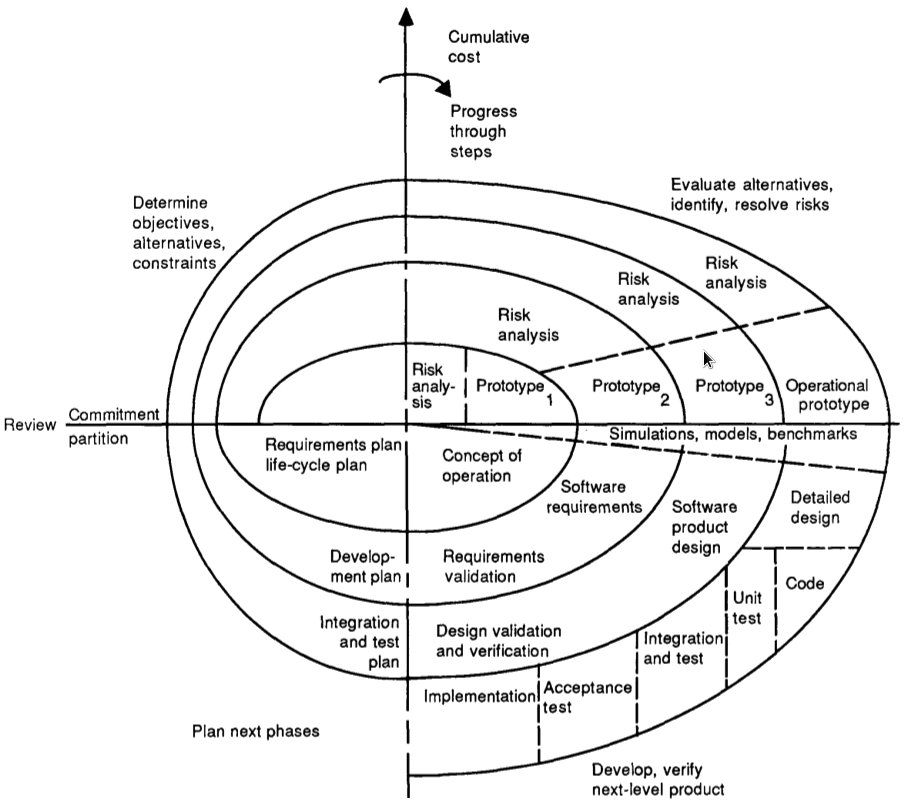
\includegraphics[width=.8\textwidth]{software-engineering/project-management/process/sdlc/spiral/spiral}
		\end{block:fact}
	\end{columns}
	
	\begin{block:fact}{Riscos}
		\begin{itemize}
			\item Avaliar as opções em relação aos objetivos e às restrições.
			\item Identificar riscos a partir da avaliação feita.
			\item Identificar outros riscos.
			\item Determinar a causa dos riscos (por análise, prototipação, \ldots).
		\end{itemize}
	\end{block:fact}

	\note{
		\begin{itemize}
			\item Recursos humanos inadequados
			\item Orçamento e prazos irrealísticos
			\item Requisitos de software incorretos
			\item Interface de usuário incorreta
			\item Perfeccionismo (\foreign{gold plating})
			\item Volatilidade de requisitos
			\item Deficiências de componentes externos necessários ao projeto
			\item Deficiências em tarefas executadas por terceiros
			\item Desempenho inadequado
			\item Baixa capacidade técnica
		\end{itemize}
	}
\end{frame}


\begin{frame}
	\frametitle{Modelo espiral}
	\framesubtitle{Terceiro quadrante -- Desenvolvimento}

	\begin{columns}
		\column{.48\textwidth}
		\begin{block:fact}{Terceiro quadrante}
			\begin{itemize}
				\item A partir dos riscos existentes, desenvolver o produto de modo a
				tratar os principais riscos.
			\end{itemize}
		\end{block:fact}

		\column{.48\textwidth}
		\begin{block:fact}{}
			\centering
			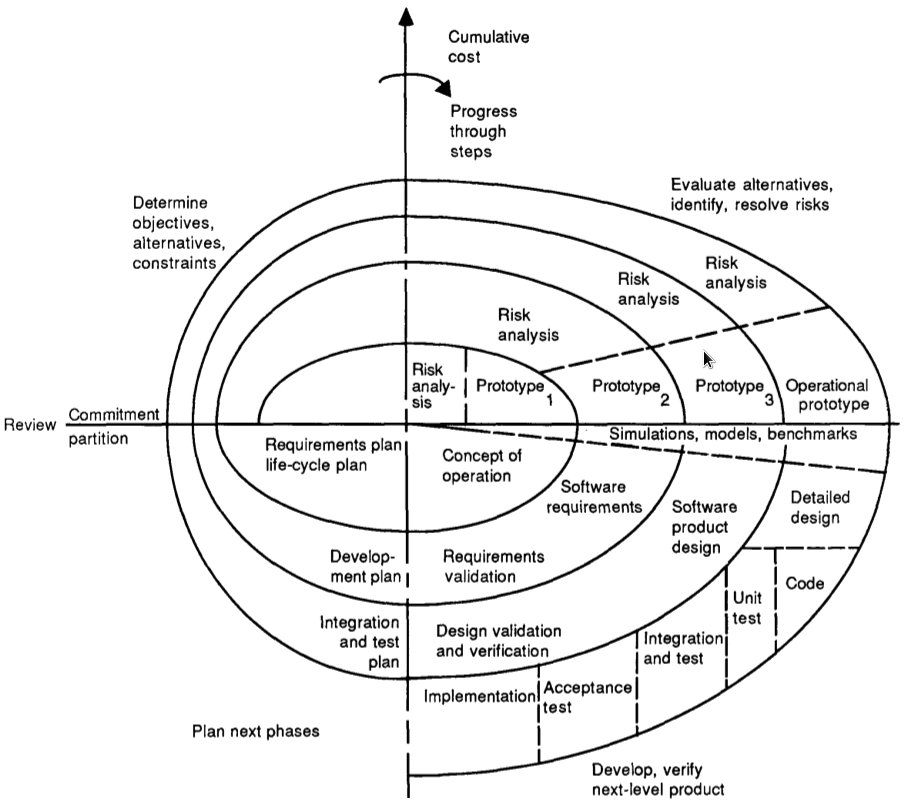
\includegraphics[width=\textwidth]{software-engineering/project-management/process/sdlc/spiral/spiral}
		\end{block:fact}
	\end{columns}
\end{frame}


\begin{frame}
	\frametitle{Modelo espiral}
	\framesubtitle{Quarto quadrante -- Planejamento}

	\begin{columns}
		\column{.48\textwidth}
		\begin{block:fact}{Quarto quadrante}
			\begin{itemize}
				\item Revisar os artefetos.
				\item Planejar a próxima iteração.
			\end{itemize}
		\end{block:fact}

		\column{.48\textwidth}
		\begin{block:fact}{}
			\centering
			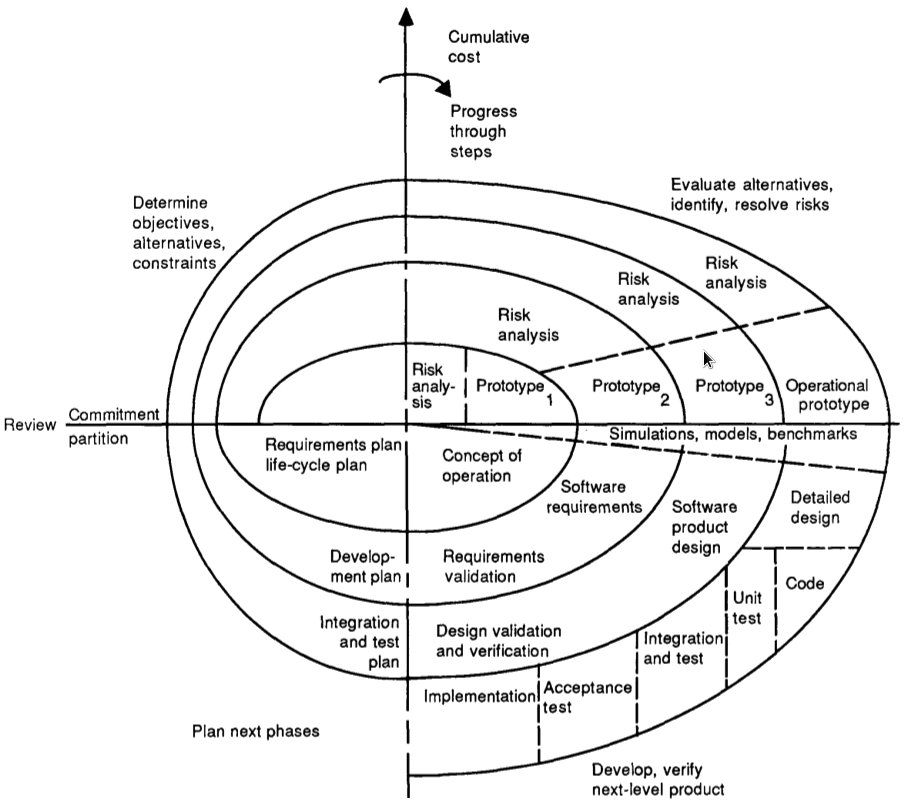
\includegraphics[width=\textwidth]{software-engineering/project-management/process/sdlc/spiral/spiral}
		\end{block:fact}
	\end{columns}
\end{frame}


\begin{frame}
	\frametitle{Modelo espiral}
	\framesubtitle{Exemplo}

	\begin{columns}
		\column{.48\textwidth}
		\begin{block:fact}{Iteração 0}
			\centering
			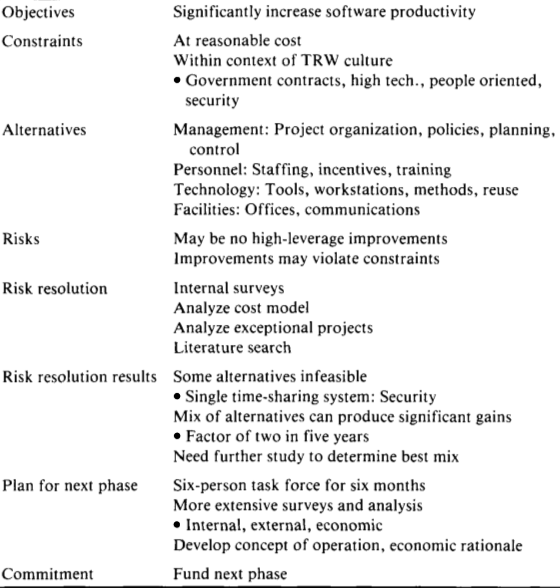
\includegraphics[width=\textwidth]{software-engineering/project-management/process/sdlc/spiral/spiral-trw-round0-riskmanagement}
		\end{block:fact}

		\column{.48\textwidth}
		\begin{block:fact}{Iteração 3}
			\centering
			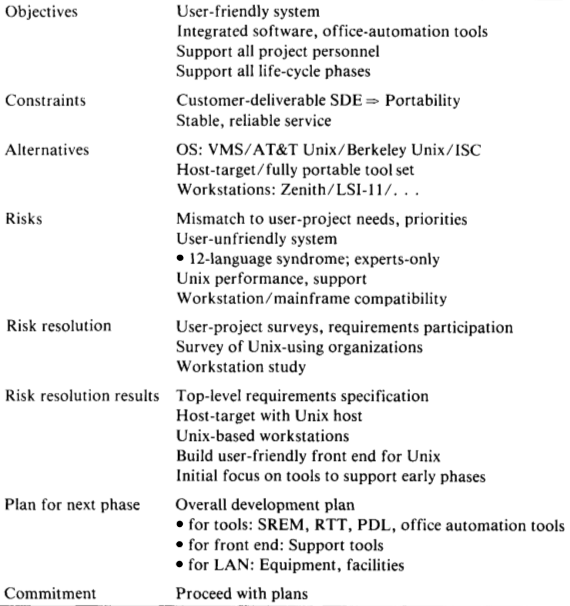
\includegraphics[width=\textwidth]{software-engineering/project-management/process/sdlc/spiral/spiral-trw-round3-riskmanagement}
		\end{block:fact}
	\end{columns}
\end{frame}


\begin{frame}
	\frametitle{Modelo espiral}
	\framesubtitle{Condições para encerramento}

	\begin{columns}
		\column{.48\textwidth}
		\begin{block:fact}{Encerramento da espiral}
			\begin{itemize}
				\item Falha em alcançar o objetivo.
				\item Sucesso em alcançar o objetivo (embora nesse caso possa ser iniciada
				nova iteração para, por exemplo, manutenção).
			\end{itemize}
		\end{block:fact}

		\column{.48\textwidth}
		\begin{block:fact}{}
			\centering
			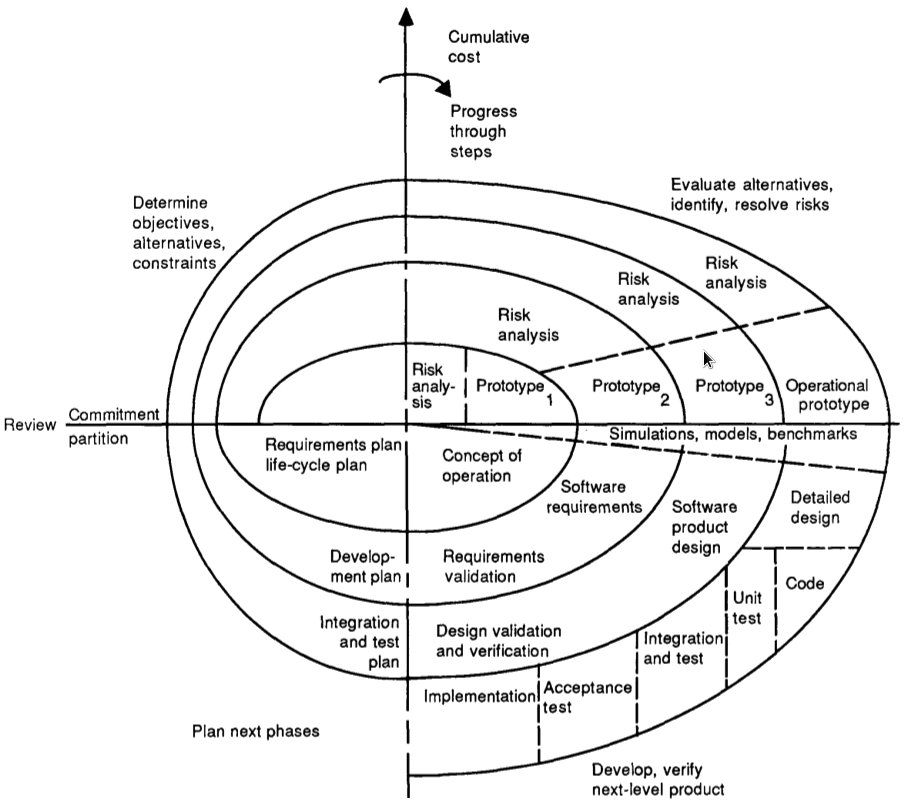
\includegraphics[width=\textwidth]{software-engineering/project-management/process/sdlc/spiral/spiral}
		\end{block:fact}
	\end{columns}
\end{frame}


\begin{frame}[hasnext=false, hasprev=true]
	\frametitle{Modelo espiral}
	\framesubtitle{Considerações finais}

	\begin{block:fact}{Pontos positivos}
		\begin{itemize}
			\item Riscos são tratados o quanto antes, aumentando a chance do projeto
			ser bem sucedido.
			\begin{itemize}
				\item É equivalente ao cascata se o projeto é de baixo risco ou possui
				risco elevado
			\end{itemize}
			
			\item Documentação ampla existe para elementos associados com grande risco
			ao projeto (para os demais existe pouca documentação).
			
			\item Desta forma, demanda-se menos esforço dos especialistas para fazer
			a documentação (esforço que pode ser utilizado em outras tarefas de
			desenvolvimento).
		\end{itemize}
	\end{block:fact}

	\begin{block:fact}{Pontos negativos}
		\begin{itemize}
			\item Depende da capacidade de gerenciamento de riscos da organização.
		\end{itemize}
	\end{block:fact}
\end{frame}
